\documentclass[12pt,a4paper,openany,oneside]{book}

%%%%%%%%%%%%%%%%%%%%%%%%
% Imports
%%%%%%%%%%%%%%%%%%%%%%%%
\usepackage[utf8]{inputenc}
\usepackage[italian]{babel}
\usepackage{minted}
\usepackage{hyperref} % Extensive support for hypertext in LATEX (https://ctan.org/pkg/hyperref)
\usepackage{csquotes}
\usepackage{graphicx} % Enhanced support for graphics (https://ctan.org/pkg/graphicx)
\usepackage{framed} % Framed or shaded regions that can break across pages (https://ctan.org/pkg/framed)
\usepackage[acronyms,style=altlist,nopostdot]{glossaries}
\usepackage[font=small,labelfont=bf,tableposition=top]{caption}
\usepackage[style=numeric,useprefix,hyperref,backend=bibtex,sorting=none]{biblatex} % Sophisticated Bibliographies in LATEX (https://ctan.org/pkg/biblatex)
\usepackage{subfig}
\usepackage{forest} % Drat tree like data structures (https://ctan.org/pkg/forest)

%%%%%%%%%%%%%%%%%%%%%%%%
% Settings
%%%%%%%%%%%%%%%%%%%%%%%%
\providecommand*{\listingname}{Cod.}
\renewcommand*{\figureautorefname}{Fig.}
\renewcommand*{\chapterautorefname}{Cap.} 
\renewcommand*{\sectionautorefname}{Sez.} 
\renewcommand*{\subsectionautorefname}{Sub-sec.} 
\renewcommand*{\listingscaption}{Codice}
\graphicspath{ {./img/} } % Base image path
\setminted{fontsize=\footnotesize,breaklines,tabsize=1}

%%%%%%%%%%%%%%%%%%%%%%%%
% References
%%%%%%%%%%%%%%%%%%%%%%%%
\addbibresource{resources.bib} %Import the bibliography file

%%%%%%%%%%%%%%%%%%%%%%%%
% Glossary
%%%%%%%%%%%%%%%%%%%%%%%%
\makeglossaries
\loadglsentries{glossary}

%%%%%%%%%%%%%%%%%%%%%%%%
% Begin document
%%%%%%%%%%%%%%%%%%%%%%%%
\begin{document}

% Metadata
\title{EWT summary}
\author{Ernesto Casablanca}
\date{\today}

% Title page
\begin{titlepage}
    \centering
    
\includegraphics[width=2.434cm,height=2.565cm]{university_logo.png}

    \bigskip

    {\Large \textbf{UNIVERSIT\`A DEGLI STUDI DI CATANIA}}

    {\scshape
        \large
        Dipartimento di Matematica e Informatica
    }
    {\scshape
        \normalsize
        Corso di Laurea Triennale in Informatica
    }

    \bigskip

    \hrule

    \bigskip
    \bigskip
    \bigskip
    \bigskip

    {\itshape
        \large
        Ernesto Casablanca
        \par}

    \bigskip
    \bigskip
    \bigskip
    \bigskip

    {\centering
        \Large
        Decentralizzazione del mercato dell'energia
        \par}
    {\centering
        Decentralization of the energy market
        \par}

    \bigskip
    \bigskip
    \bigskip
    \bigskip
    \bigskip
    \bigskip

    \begin{minipage}[b]{8 cm}
        \hrule
        \bigskip
        {\centering\scshape
            Relazione Progetto Finale
            \par}
        \bigskip
        \hrule
    \end{minipage}

    \bigskip
    \bigskip
    \bigskip
    \bigskip
    \bigskip
    \bigskip
    \bigskip
    \bigskip
    \bigskip
    \bigskip
    \bigskip

    {\raggedleft
        Relatore: Prof. Giuseppe Pappalardo \\
        Correlatore: Dott. Giovanni Marotta
        \par}

    \bigskip
    \bigskip
    \bigskip
    \bigskip

    \hrule

    \bigskip

    {\centering
        Anno Accademico 2020 - 2021
        \par}

\end{titlepage}


% Index
\tableofcontents

% Abstract
\chapter*{Abstract}
\addcontentsline{toc}{chapter}{Abstract} % add the chapter to the index

%%%%%%%%%%%%
% Content
%%%%%%%%%%%%
Il mondo della produzione e distribuzione dell'energia elettrica sta andando incontro ad un processo di decentralizzazione sempre più rapido. \\
La spinta nasce dall'ingresso nel mercato di nuovi piccoli produttori di energia rinnovabile con capacità variabili e
da una domanda che necessita di sempre più flessibilità e con una rinnovata sensibilità ambientale. \\
Per poter supportare questo nuovo tipo di mercato, incentrato su un rapporto più diretto fra produttore e consumatore,
diversi progetti hanno preso in considerazione la tecnologia delle blockchain, sfruttandone i punti di forza e cercando di superarne le limitazioni. \\
L'utente ottiene anche un controllo maggiore ha sulle informazioni che fornisce, ottenendo inoltre le garanzie di integrità e non ripudio che le tecnologie
crittografiche combinate con la blockchain sono in grado di fornire. \\
In questo documento ci si concentrerà particolarmente sulle soluzioni in questo ambito proposte dal progetto Energy Web,
al fine di fornire un esempio concreto di una possibile implementazione. \\
I concetti chiave possono comunque essere applicati ad altri progetti della stessa natura.

% Introduction
\chapter{Introduzione}

%%%%%%%%%%%%
% Content
%%%%%%%%%%%%
\section{Il mercato dell'energia}
La gestione centralizzata della rete elettrica è stata a lungo la scelta più ragionevole, ma adesso ha senso rivedere questo paradigma.
In passato, i grandi operatori elettrici erano anche quelli che producevano anche la quasi totalità dell'energia, gli unici ad avere a disposizione i mezzi per realizzare impianti costosi e complessi.
Ad effettuarne poi la distribuzione sono poi i \gls{tso}, spesso con coperture nazionali, come la italiana Terna \cite{art:terna-role}. \\
La situazione odierna, tuttavia, è diversa.
Negli anni abbiamo assistito ad una riduzione progressiva del costo degli impianti per la produzione di energia rinnovabile,
anche grazie a regolamentazioni estremamente favorevoli \cite{art:renewable-energy-regulations}. \\
La conseguenza è una diffusione sempre più capillare di piccoli produttori di energia elettrica,
che attraverso piccoli impianti, spesso domestici, sono in grado di offrire un contributo attivo alla rete \cite{art:renewable-energy-increment}. \\
Ad essi si aggiungono dispositivi come veicoli elettrici e nuovi sistemi di stoccaggio di energia, i quali, se ben gestiti,
possono offrire un servizio utile all'intera rete elettrica. \\
Tutti questi dispositivi, definiti \gls{der}, introducono la necessità di un flusso bidirezionale di energia che li includa come agenti attivi \cite{art:enel-der}. \\
Inoltre, la natura variabile e difficile da prevedere della maggior parte delle fonti di energia rinnovabile o \gls{res} ne richiede una gestione flessibile,
in grado di garantire robustezza e stabilità all'intera rete \cite{art:blockchain-der}. \\

La gestione di queste piccole realtà, mal si sposa con l'attuale struttura centralizzata, e impone un cambio di paradigma verso un'architettura distribuita,
in grado di includere i \gls{der} e mettere a più stretto contatto produttore e consumatore.

\begin{figure}[h]
    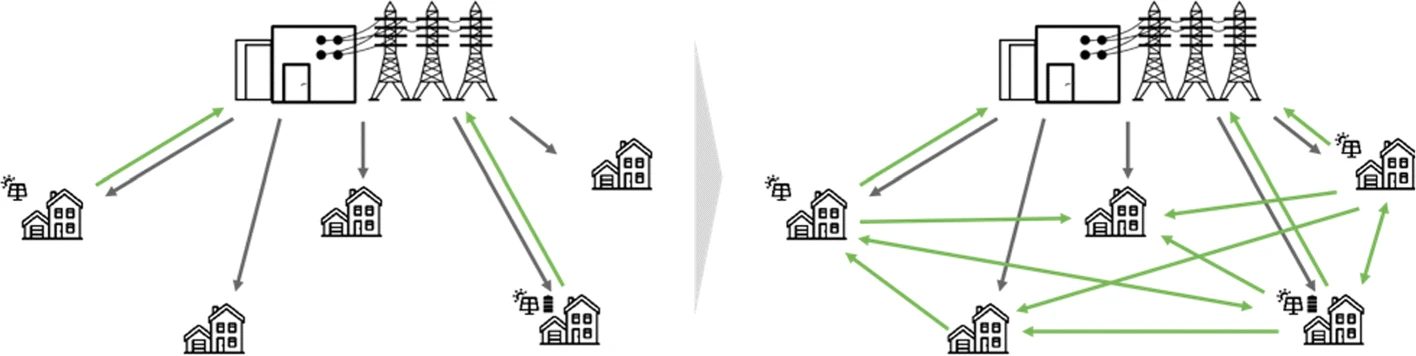
\includegraphics[width=9cm]{p2pgrid}
    \centering
    \caption{Da rete da centralizzata a rete distribuita \cite{img:p2pgrid}}
    \label{lab:p2pgrid}
\end{figure}


\section{La tecnologia delle blockchain}
La tecnologia delle blockchain esiste già da parecchi anni, ma negli ultimi tempi ha ricevuto crescenti attenzioni da studiosi e industrie, intenzionate a sfruttarne a pieno il potenziale. \\
Tralasciando i dettagli più tecnici della tecnologia, che è possibile approfondire in pubblicazioni come quelle referenziate in \cite{art:blockchain} e \cite{art:blockchain-for-industry},
la blockchain può essere vista come una lista di transazioni pubblica, decentralizzata e immutabile, se non per l'aggiunta di nuove transazioni, della quale chiunque può possedere una copia. \\
L'integrità e la correttezza delle transazioni vengono garantite dagli algoritmi crittografici, che rendono molto facile verificare la validità della transazione. \\
Ciò permette l'interazione di una qualsiasi entità con le altre senza che questa debba fare affidamento su nient'altro che l'algoritmo di consenso distribuito che governa la blockchain, eliminando la necessità di un intermediario fra le parti.
Il risultato è una rete distribuita \gls{p2p} estremamente robusta che si presta a molteplici applicazioni. \\
A rendere ancora più appetibile questa tecnologia sono gli smart contracts, presenti in reti come Ethereum \cite{wiki:eth-smart-contracts}. Semplificando, si tratta di veri e propri software rilasciati sulla blockchain
in grado di compiere svariate azioni in maniera automatica seguendo la loro programmazione.

% Energy web
\chapter{Energy web}

%%%%%%%%%%%%
% Content
%%%%%%%%%%%%
\section{Cos'è Energy Web}
\gls{ew} è un progetto nato nel 2017 con sede in Zugo, Svizzera \cite{wiki:ew-history}.
Ad affiancarlo e dargli valore vi sono molti partner commerciali, comprese aziende molto conosciute nel settore energetico \cite{wiki:ew-affiliate}. \\
L'obiettivo prefissato da \gls{ew} è quello di spingere per uno sviluppo del settore che punti verso un abbassamento delle emissioni di carbonio e che sia in grado di gestire la decentralizzazione del mercato delle risorse.
Per farlo, \gls{ew} utilizza tecnologie distribuite e open-source dalle quali partire per realizzare un'infrastruttura commerciale specifica per l'ambito energetico \cite{wiki:ew-about}. \\
Nel 2019, \gls{ew} ha rilasciato \gls{ewc}, una blockchain pubblica basata su Ethereum, sulla quale si basa l'intero ecosistema di \gls{ew}: \gls{ewdos}.

\section{EW-DOS}
Il cuore del progetto di \gls{ew} è \gls{ewdos}, un'infrastruttura digitale open-source ad accesso pubblico e decentralizzato. \\
L'idea è quella di fornire un insieme di strumenti e servizi che rendano il più semplice possibile lo sviluppo di \gls{dapp} mirate al settore energetico,
anche se, ovviamente, le varie tecnologie possono essere applicate anche ad ambiti più generici. \\
L'intero sistema è stato pensato come tre strati sovrapposti, in cui ogni strato si basa su quello sottostante per implementare ulteriori funzionalità, come mostrato in \autoref{lab:ew-dos}. \\

I tre strati sono:
\begin{itemize}
    \item Trust - \gls{ewc}
    \item Utility - Servizi e astrazioni sopra la blockchain
    \item Toolkit - Frameworks e toolkit per la costruzione di applicazioni
\end{itemize}

\begin{figure}[h]
    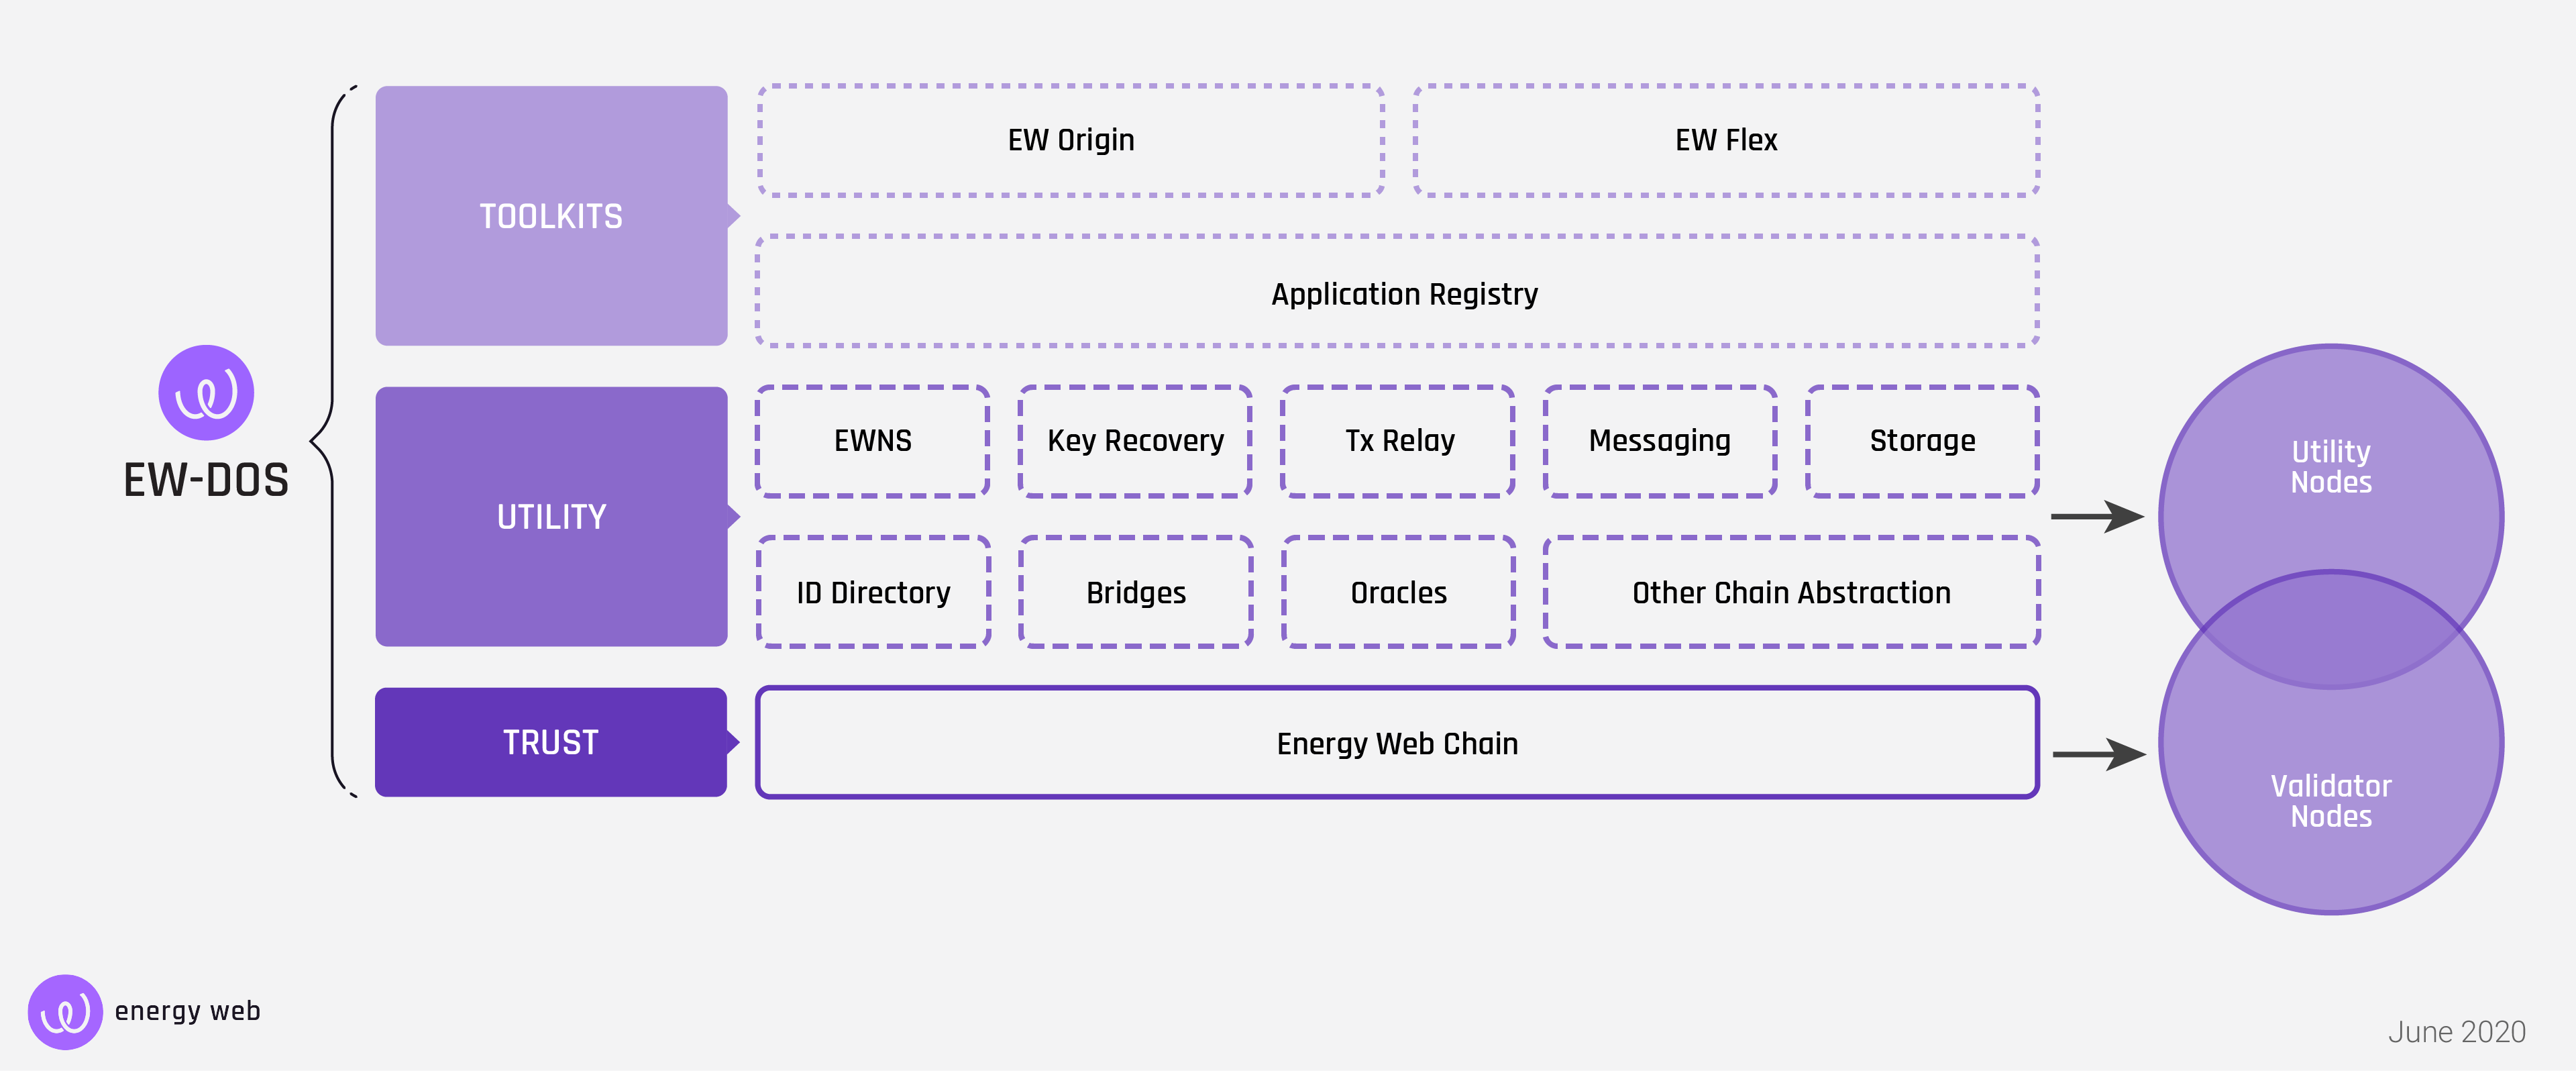
\includegraphics[width=13cm]{ew-dos}
    \centering
    \caption{Visualizzazione della struttura di \gls{ewdos} \cite{img:ew-dos}}
    \label{lab:ew-dos}
\end{figure}

\section{Trust}
Il livello Trust comprende la \gls{ewc} (cfr. \autoref{cap:ewc}),
il cui ruolo principale è quello di assicurare che ci sia consenso sui dati e che tutte le applicazioni e gli smart contracts si comportino in maniera deterministica. \\
Si tratta di una blockchain basata su Ethereum, \gls{evm} inclusa, e rispetta tutti gli \gls{erc}. \\
Il token digitale per il pagamento delle transazioni e dei servizi offerti dalla piattaforma è l'\gls{ewt} e l'algoritmo di consenso è il \gls{poa}. \\
È presente anche una test-net, chiamata Volta, usata per testare i progetti e le applicazioni prima di lanciarle sulla main-net.

\section{Utility}
Il livello di utility è composto da un insieme di servizi basati sulla \gls{ewc} che hanno lo scopo di rendere quanto più accessibile e invitante possibile l'intera infrastruttura per gli sviluppatori di DApp.
Comprende un gran numero di smart contracts per il back-end e di librerie per il front-end \cite{art:ew-dos}. \\
Come anticipato, il pagamento di servizi del livello di Utility della piattaforma vengono pagati in \gls{ewt}. \\
I nodi della blockchain che forniscono queste funzionalità sono chiamati Utility Nodes, e vengono ricompensati attraverso il meccanismo dello Staking (cfr. \autoref{sec:staking}).\\

I servizi riguardano principalmente il fornire protocolli condivisi e soluzioni per l'identità, la comunicazione e lo scambio di informazioni.
Questi obiettivi sono raggiunti tramite:
\begin{itemize}
    \item \textbf{\gls{iam}}: servizio di autenticazione e autorizzazione basato sull'identità utilizzabile da qualsiasi \gls{dapp} in maniera trasparente all'utente
    \item \textbf{Messaggistica decentralizzata}: servizi di comunicazione fra agenti che operano a livelli diversi della rete elettrica
    \item \textbf{Servizi di storage e \gls{ens}}: servizi di storage distribuiti off-chain e nomi di dominio per migliorare l'esperienza utente
\end{itemize}

\section{Applicazioni e Toolkit}
Il livello toolkit comprende una serie di \gls{sdk}, framework ed applicazioni di esempio utili per realizzare \gls{dapp} che sfruttino al massimo le funzionalità di \gls{ewdos} \cite{art:ew-dos}.
Sebbene siano pensati per il settore energetico, la loro natura open-source li rende ottime basi di partenza per costruire soluzioni anche per altri ambiti.

\subsection{Origin Core}
Framework per sviluppare applicazioni che supportino il tracciamento, la trasmissione e il conferimento di \gls{eac} alle \gls{res} secondo gli standard del settore.

I due attori principali sono il Registry e l'Issuer.
Il primo salva e amministra le informazioni legate ad utenti e \gls{der}, con la possibilità di mantenere dati potenzialmente sensibili off-chain, cioè utilizzando dello storage al di fuori della blockchain.
Il secondo potrà essere utilizzato dalle autorità competenti per coniare nuovi \gls{eac} che siano tracciabili, con una implementazione basata sullo standard ERC-1155.

\subsection{Origin 24/7}
\gls{dapp} per il monitoraggio della generazione e del consumo di energia rinnovabile su un'elevata granularità.
Fornisce le informazioni necessarie agli utenti per acquistare \gls{eac} che rispondono alle loro necessità.

\subsection{Local Marketplace}
Marketplace che consente la registrazione di dispositivi o organizzazioni e l'emissione,
il monitoraggio e lo scambio di \gls{eac} specificamente conformi agli standard \gls{irec}.

\subsection{Zero, Zero Labs}
Infrastruttura per la promozione dell'adozione di energia a zero-carbon,
rendendo quanto più accessibile e appetibile partecipare a mercati che la trattano.
Prevede inoltre un sistema per garantire agli acquirenti una certificazione universalmente riconosciuta e facilmente consultabile \cite{art:zero-labs}.


% Energy web chain
\chapter{Energy Web chain}
\label{cap:ewc}

%%%%%%%%%%%%
% Content
%%%%%%%%%%%%
\section{Confronto con Ethereum}
Non è un mistero che la \gls{ewc} sia basata su Ethereum, più precisamente sulla sua ottava hard-fork, Istanbul \cite{wiki:ew-fork}.
È in programma una ulteriore migrazione alla hard-fork Berlino, che avverrà quanto prima \cite{wiki:ew-berlino}. \\
Anche alcuni dei servizi offerti, come l'\gls{ewns} sono fork con modifiche minime di progetti nati su Ethereum. \\

Tuttavia, ci sono alcuni aspetti in cui le due reti differiscono, come riassunto nella seguente tabella: \\

\hskip-.6cm
\begin{tabular}{||p{6cm}|p{7cm}||}
    \hline
    Problema                                                    & Modifica                                                                                                                    \\
    \hline\hline
    Basso throughput, alti costi, scalabilità limitata          & Utilizzo della \gls{poa}: incrementa il throughput fino a 30x                                                               \\
    \hline
    Poco adatta a piccoli dispositivi (IoT)                     & Maggiore focus sui \textbf{light client} per connettere anche piccoli dispositivi (\gls{iot})                               \\
    \hline
    Nessuna distinzione fra i nodi con diverse autorizzazioni   & È possibile differenziare fra nodi con compiti ed autorizzazioni diverse                                                    \\
    \hline
    Difficoltà a gestire transazioni che necessitino di privacy & Possibilità di mantenere i dati privati integrando protocolli crittografici e appoggiandosi a storage esterni, se richiesto \\[1ex]
    \hline
\end{tabular}

\section{Testnet}
Energy Web mette a disposizione una testnet che permette a chiunque sia interessato alle peculiarità della loro offerta di testare tutti i servizi senza spendere token reali. \\
La testnet si chiama Volta, e non è dissimile alle testnet che affiancano Ethereum. \\

Di seguito le differenze fra Volta e la \gls{ewc} \cite{wiki:ew-two-networks}:\\

\hskip-.6cm
\begin{tabular}{||p{4cm}|p{5cm} p{5cm}||}
    \hline
                       & Volta                                               & EWC                                                     \\ [0.5ex]
    \hline\hline
    Data di lancio     & Aprile 2019                                         & Giugno 2019                                             \\
    \hline
    Funzione primaria  & Pre-produzione                                      & Produzione                                              \\
    \hline
    Token              & 90M + 10M di compensi \newline transazioni e faucet & 90M + 10M di compensi \newline transazioni              \\
    \hline
    Tariffe            & Le risorse usate non hanno valore monetario         & Valore monetario delle transazioni in base al gas usato \\
    \hline
    Caratteristiche    & 5 secondi per block \newline limite di 8M gas       & 5 secondi per block \newline limite di 8M gas           \\
    \hline
    Connessione ad ETH & Bridge su Kovan Test Net                            & Bridge su Ethereum main-net con un ERC-20 token         \\
    \hline
    Nodi validatori    & 3 al lancio \newline max 150                        & 10 al lancio \newline max 150                           \\ [1ex]
    \hline
\end{tabular}

\section{Algoritmo di consenso Proof of Authority}
L'algoritmo che permette di assicurare un consenso sullo stato della blockchain fra tutti i nodi è \gls{poa}, più precisamente l'algoritmo Aura \cite{art:aura}\cite{wiki:poa}. \\
Nel caso di \gls{ewc}, i nodi validatori sono gestiti dai partner dell'associazione.
Si tratta, nella maggior parte dei casi, di aziende leader del settore energetico. \\
In breve, il funzionamento è il seguente:

\begin{enumerate}
    \item Tutti i nodi validatori possiedono una lista aggiornata degli altri nodi validatori, oltre alla copia completa della blockchain e ad alcuni meta-dati ad essa collegati (es. il throughput della blockchain)
    \item Per una finestra temporale ben definita, un validatore primario viene scelto dall'algoritmo e svolge il compito di raccogliere le transazioni e produrre il nuovo blocco. La scelta del validatore primario è in funzione del timestamp e del numero di validatori
    \item Se il validatore primario non riesce a produrre il blocco (es. problemi hardware) o il blocco non viene convalidato dagli altri nodi (es. problemi di connessione), il prossimo validatore primario riprenderà dalle transazioni rimaste in sospeso
    \item Gli altri validatori controllano che le transazioni siano legittime e firmano il blocco per poi propagarlo alla rete
    \item Se la maggioranza dei validatori ha verificato il blocco, questo è aggiunto alla blockchain
\end{enumerate}


\begin{figure}[ht]
    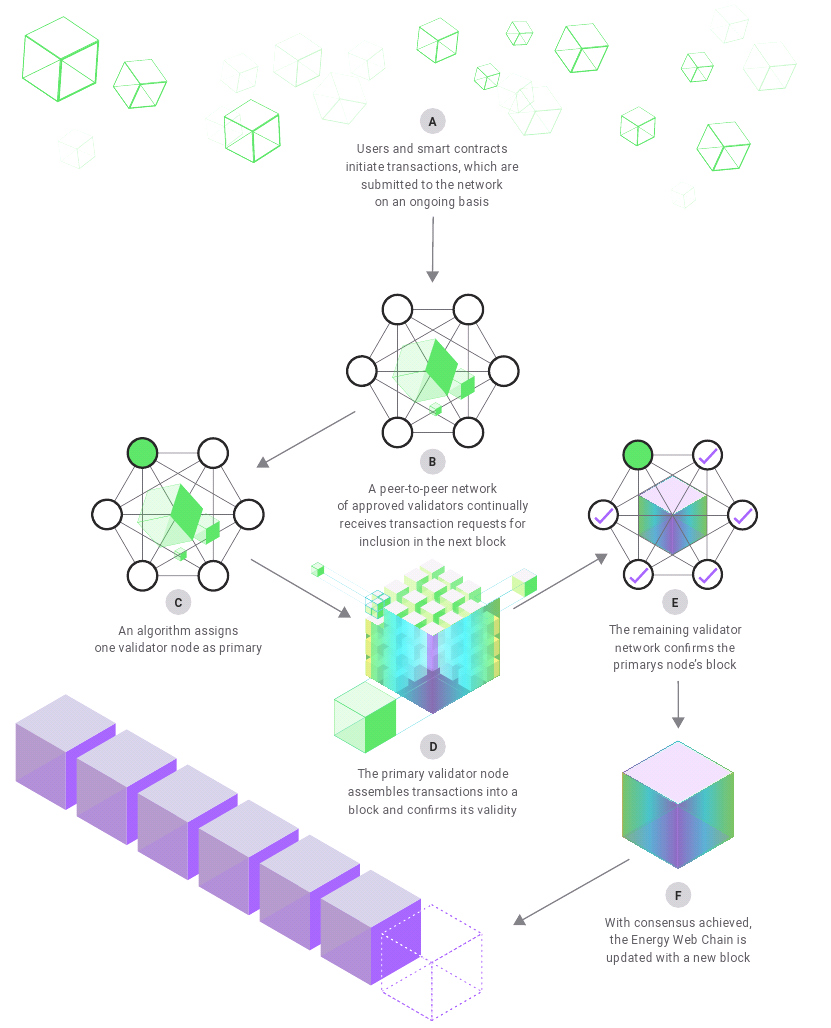
\includegraphics[height=14cm,keepaspectratio]{ew-poa}
    \centering
    \caption{Passi dell'algoritmo \gls{poa} \cite{img:ew-poa}}
    \label{lab:ew-poa}
\end{figure}

\subsection{Smart-contract di sistema}
Gli smart-contract di sistema sono una collezione di smart-contract già presenti su \gls{ewc} che implementano il protocollo di consenso \gls{poa}.
Il codice che li compone è pubblico e consultabile nella \href{https://github.com/energywebfoundation/ewc-system-contracts}{repository GitHub}.
Sintetizzando, vi sono tre smart-contract principali:

\begin{itemize}
    \item \href{https://energy-web-foundation.gitbook.io/energy-web/technology/the-stack/trust-layer-energy-web-chain/system-architecture/system-contracts/validator-set-contract#overview}{\textbf{Validator Set Contracts}}: gestisce i permessi e il comportamento del validatore
    \item \href{https://energy-web-foundation.gitbook.io/energy-web/technology/the-stack/trust-layer-energy-web-chain/system-architecture/system-contracts/block-reward-contract}{\textbf{Reward Contracts}}: gestisce la ricompensa dovuta al validatore
    \item \href{https://energy-web-foundation.gitbook.io/energy-web/technology/the-stack/trust-layer-energy-web-chain/system-architecture/system-contracts/holding-contract#overview}{\textbf{Holding Contracts}}: distribuisce i \gls{ewt} iniziali
\end{itemize}

\section{Costi di transazione}
Una transazione è una qualsiasi operazione che modifica lo stato della blockchain. Trasferire token fra account, creare un nuovo smart contract o modificarne lo stato sono esempi di transazioni. \\
Ogni transazione ha un costo che sarà pagato in \gls{ewt}.
Grazie alla specificità di utilizzo della \gls{ewc} e all'algoritmo di consenso, che insieme contribuiscono a ridurre la congestione della rete aumentandone il throughput,
le tariffe sono generalmente molto basse e vanno da $0.00001$ a $000000.1$ \gls{ewt} \cite{art:manage-costs}. \\
Il costo monetario da pagare per poter effettuare una transazione lo si può calcolare a partire dai seguenti fattori:

\begin{itemize}
    \item \textbf{Il costo in gas:} il gas rappresenta la complessità computazionale necessaria per risolvere la transazione. Più è complessa l'operazione più gas sarà richiesto
    \item \textbf{Prezzo del gas:} valore dell'unità di gas in EWT. Prima di effettuare una transazione, l'utente stabilisce quanto è disposto a pagare per unità di gas. Più è alta l'offerta, maggiore sarà la priorità della transazione
    \item \textbf{Valore di mercato del token:} se si vuole ottenere il costo della transazioni in moneta fiat, basta effettuare la conversione fra EWT spesi e il loro valore monetario
\end{itemize}

Riassumendo con una formula \cite{wiki:ew-transaction-cost}: \\
$ costo(\$) = costo\ gas(gas) * prezzo\ gas(token/gas) * valore\ token (\$/token) $.

\subsection{Precise Proofs}
Precise Proofs è uno schema basato sugli alberi di Merkle (cfr. \autoref{sec:merkle-tree}), in grado di verificare l'autenticità della struttura dati rivelando solo un subset di dati. \\
Si parte realizzando un albero di Merkle a partire dai dati interessati e si rende pubblica la radice. \\
Un terzo ente, interessato a verificare la validità di un subset di dati, riceverà solo i dati effettivamente richiesti e le hash dei dati non necessari.
In questo modo si hanno abbastanza informazioni da poter ricostruire la radice minimizzando i dati resi pubblici.

\subsection{Zero Knowledge Proof Protocols}
Gli Zero Knowledge Proof Protocols sono una categoria di protocolli con lo scopo di validare una computazione senza rivelarne alcun input (es. validare una transazione senza rivelare mittente, destinatario, movimento etc.).

\subsubsection{zkSNARKs}
zkSNARKs è probabilmente il protocollo più avanzato in questa categoria, sviluppato dal team Zcash \cite{wiki:zkSNARKs}.
Sebbene sia il più maturo, presenta un tallone d'Achille non indifferente. \\
Per poter utilizzare la Zero Knowledge Proof è necessario realizzare un circuito aritmetico che rappresenta la computazione da provare e generare da quello una coppia di chiavi prover/verifier.
La creazione di questo setup deve essere sicura e pattuita a priori, perché se dovesse essere compromesso un avversario potrebbe approfittarne per realizzare prove false.

\section{Storage}
Il fatto che tutti i dati siano immagazzinati sulla blockchain per essere accessibili si traduce in un incremento della memoria necessaria per salvare l'intera blockchain su un dispositivo fisico,
in una maggiore congestione della rete con conseguente calo di prestazione e in un aumento di costi possibilmente evitabili nelle esecuzione degli smart contract. \\
Una prima soluzione è di evitare di immettere dati sulla blockchain, e limitarsi ad utilizzare gli hash degli stessi, per poi limitarsi a verificarne la validità off-chain. \\
Nei casi in cui il salvataggio dei dati fosse necessario, si può provare ad optare per una delle tante soluzioni che offrono un servizio di storage distribuito. \\
Le principali soluzioni sono \gls{ipfs} e Storj.
Per una lista completa è possibile consultare la documentazione \cite{wiki:ew-storage}

\subsection{InterPlanetary File System (IPFS)}
\gls{ipfs} \cite{prod:ipfs} è un modello di filesystem distribuito.
Invece di indirizzare i file con la loro locazione, li si identifica con un hash ottenuto dal loro contenuto.
Se il file è troppo grande, lo si spezza in più parti con lo stesso risultato. \\
I nodi che fanno parte di questa rete si auto-iscrivono in delle tabelle di \gls{dht} che tengono traccia dei nodi che possiedono il file associato ad uno specifico hash. \\
Se si vuole contribuire alla rete, una volta scaricato il file lo si tiene in cache, fornendolo ad altri utenti che lo richiedano. \\
Il fatto che un file sia identificato dal suo hash garantisce inoltre l'integrità del dato e la sua immutabilità.
Per aggiornare un file, infatti, bisogna utilizzare il sistema di versioning previsto dal protocollo. \\ \\

\subsubsection{\gls{vc} su \gls{ipfs}}
Nell'ecosistema di \gls{ew} le \gls{vc} sono memorizzate su \gls{ipfs} come hash. 
Il riferimento viene mantenuto dal \gls{did} document corrispondente attraverso un service endpoint, previsto nello standard \cite{wiki:did}. 
In altre parole, i service endpoint sono ciò che collega il \gls{did} document alle proprie \gls{vc}. \\
Per poterle leggere, le \gls{vc} devono essere quindi ottenute da \gls{ipfs} e decodificate. \\
\gls{ew} fornisce una libreria javascript, \href{https://github.com/energywebfoundation/ew-did-registry/tree/development/packages/claims}{\textit{claims}}, in grado di assolvere proprio questa funzione.

\subsection{Storj}
Storj \cite{prod:storj} è molto simile ad IPFS, con l'incentivo che i nodi sono pagati per svolgere la loro funzione di content-storage.
Ovviamente il contratto prevede che l'host sia in grado fornire su richiesta in qualsiasi momento tutti i file che afferma di possedere.

\section{Governance}
La natura decentralizzata della blockchain rende un qualsiasi cambiamento che riguarda la sua infrastruttura un problema non banale. \\
Per gestire al meglio i possibili aggiornamenti che la \gls{ewc} potrebbe necessitare, si è deciso di affidarsi a chi la comprende bene, cié gli sviluppatori.
Il diritto di voto che determina quali proposte di modifica vengano accolte e quali respinte sarà determinato dalla quantità di gas che un singolo sviluppatore riesce a "generare" con i propri smart contracts.
L'idea è che il valore che lo sviluppatore fornisce all'intero sistema rappresenta il suo peso nella votazione \cite{wiki:ew-governance}. \\
Ciò non esclude che, in caso si renda necessario, alcune scelte troppo complesse possano essere prese da persone designate senza passare per il meccanismo di voto della blockchain.

\begin{figure}[h]
    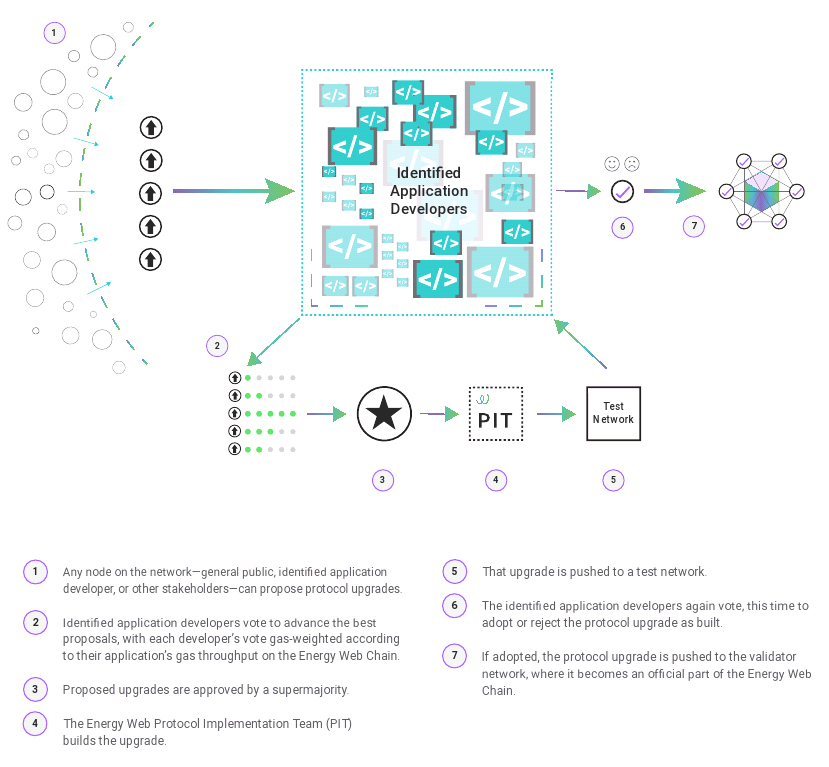
\includegraphics[height=10cm,keepaspectratio]{ew-governance}
    \centering
    \caption{Passi per l'approvazione di una modifica all'infrastruttura di \gls{ewc} \cite{img:ew-governance}}
    \label{lab:ew-governance}
\end{figure}

\section{Staking}
\label{sec:staking}
Per fornire quello che nell'architettura di ES-DOS è chiamato "Utility layer", è necessario il contributo di operatori che mettano a disposizione le proprie risorse a chi ha intenzione di sviluppare un servizio.
Perché il tutto sia affidabile e adatto ad un ambiente di produzione, devono essere garantiti dei livelli di servizio, in maniera analoga ad un qualsiasi \gls{sla} proposto da un fornitore di SaaS. \\
La soluzione proposta non è dissimile a quella implementata in altre blockchain, e si rifà al modello \gls{pos}.
Gli attori in questo modello vengono suddivisi in due categorie:

\begin{itemize}
    \item \textbf{Service providers:} sono organizzazioni che mettono a disposizione i nodi di utility.
          Per essere approvato, un service provider deve poter dimostrare la propria identità e depositare in garanzia una quantità di EWT per un periodo multi-annale.
          Dopo essere stati approvati, i service providers possono aggiungere ulteriori nodi di utility incrementando proporzionalmente il deposito di EWT.
          Finché lo \gls{sla} continua ad essere rispettato, i service providers guadagneranno un interesse in base al loro deposito.
          In questo momento, il deposito minimo necessario per essere approvati come service provider si attesta fra i $10000$ e i $100000$ EWT, a cui si aggiungono fra i $1000$ e i $10000$ EWT per service node \cite{art:ew-staking}.
    \item \textbf{Patrons:} sono gli individui o le organizzazioni che finanziano un service provider depositando dei loro EWT per il service provider.
          Differentemente rispetto a ciò che accade per i service provider, non c'è un minimo alla somma depositata e questa può essere ritirata in qualsiasi momento.
          Questo porta i patrons a favorire service provider che rispettano gli \gls{sla} e che offrano il miglior modello di revenue-sharing.
\end{itemize}

\begin{figure}[h]
    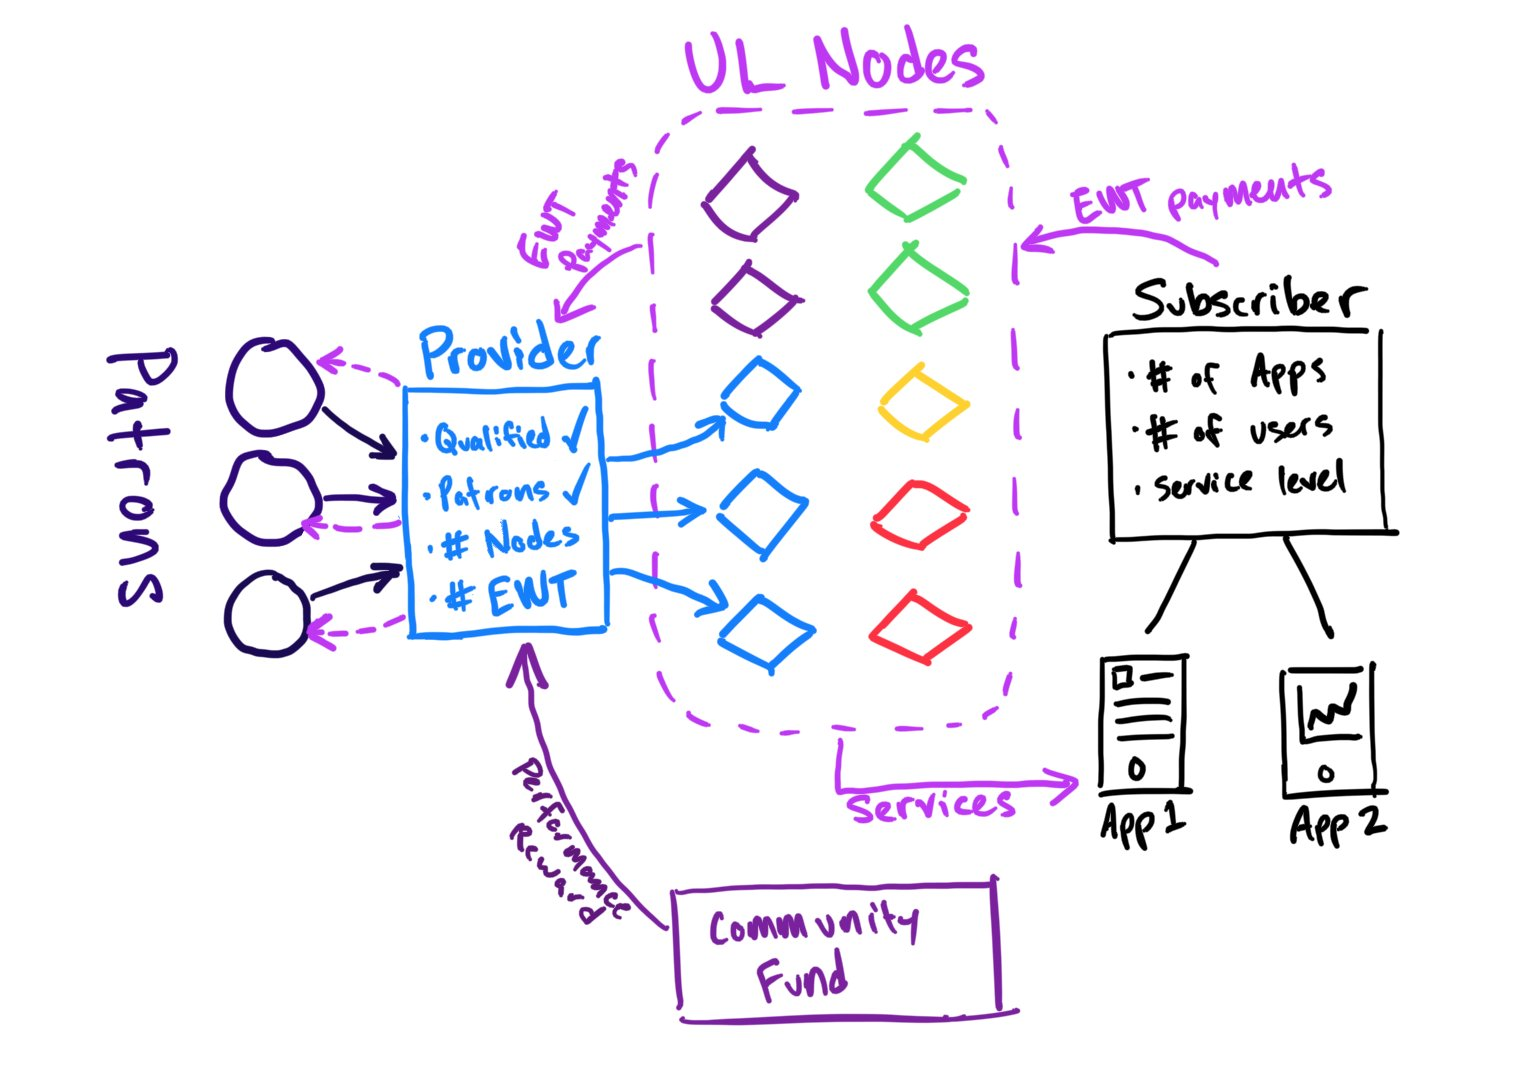
\includegraphics[height=10cm,keepaspectratio]{ew-staking}
    \centering
    \caption{Come l'utility layer supportato dallo staking si integra in EW-DOS \cite{art:ew-staking}}
    \label{lab:ew-staking}
\end{figure}

% Energy web servizi
\chapter{Servizi di Energy Web}

%%%%%%%%%%%%
% Content
%%%%%%%%%%%%
\section{Energy Web Name Service (EWNS)}
\label{sec:ewns}

L'\gls{ens} è un sistema di denominazione distribuito, aperto ed estensibile basato sulla blockchain di Ethereum, ed una sua implementazione è stata resa disponibile anche sulla \gls{ewc}. \\
Analogamente a un DNS, gli indirizzi vengono mappati su nomi di dominio facilmente memorizzabili, dando all'utente un'alternativa all'utilizzo degli indirizzi esadecimali. \\
L'implementazione disponibile pubblicamente consente prevede: indirizzi, indirizzi inversi, hash di dati, definizioni ABI, chiavi pubbliche, interfacce di smart contract e altro \cite{wiki:ewns}.

Per un utente finale il tutto è completamente trasparente.
È compito dello sviluppatore di DApp integrare le funzionalità dell'ENS. \\
Esistono diverse librerie che già supportano questa funzione, anche se potrebbe essere necessaria qualche patch manuale. \\
Il procedimento per risolvere un dominio con ENS, comunque, non è particolarmente complicato:

\begin{enumerate}
    \item Normalizzare ed applicare una funzione di hashing sul nome \cite{wiki:ens-normalize-name}.
    \item Chiamare la funzione resolver() sul registro ENS, passando l'output del passaggio 1. Ciò restituisce l'indirizzo del resolver responsabile del dominio
    \item Usando l'interfaccia del resolver, chiamare la funzione addr() sull'indirizzo del resolver restituito nel passaggio 2, passando come parametro l'hash trovato nel passaggio 1. In alternativa, se non si sta cercando un indirizzo, chiamare la funzione dell'interfaccia prevista, ad esempio text()
\end{enumerate}

\section{Decentralized IDentifiers (DIDs)}
\label{sec:did}

I \gls{did} sono identificatori univoci usati per realizzare identità digitali verificabili e decentralizzate. Sono la base per l'implementazione delle \gls{ssi} \cite{art:ssi}. \\
Il soggetto identificato può essere qualsiasi cosa: una persona, un'organizzazione o un bene fisico, per fare qualche esempio. \\
Un \gls{did} si comporta come un URI e punta ad un DID document, archiviato su un archivio pubblico permanente, come una blockchain.
Questo documento contiene tutte le caratteristiche (claims), ad esempio certificazioni o autorizzazioni, che si riferiscono al corrispettivo \gls{did}. \\
Chiunque può creare un nuovo \gls{did} in qualsiasi momento.

\begin{figure}[ht]
    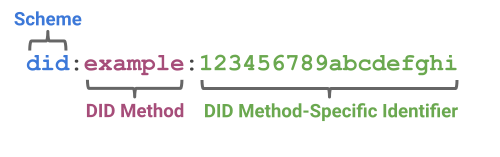
\includegraphics[width=13cm,keepaspectratio]{did-schema.png}
    \centering
    \caption{Composizione di un \gls{did} \cite{img:did-schema}}
    \label{lab:did-schema}
\end{figure}

Un \gls{did} è una stringa composta da tre parti (\autoref{lab:did-schema}): lo schema did:, un metodo e un identificatore univoco rispetto al metodo \cite{wiki:did}. \\
I documenti \gls{did}, invece, sono dei file JSON-LD \cite{wiki:json-ld}. Il documento \gls{did} contiene tutte le informazioni, o claims,
relative al soggetto identificato dal \gls{did} e fornisce una serie di meccanismi che consentono a un controller del \gls{did} di dimostrare il proprio controllo sul \gls{did}.
Tipicamente esprimono anche metodi di verifica, come chiavi pubbliche crittografiche, e servizi relativi alle interazioni con il soggetto \gls{did}. \\
Il controller di un \gls{did} è l'entità che ha la capacità di apportare modifiche a un documento \gls{did}. Questa capacità in genere è subordinata dal possesso dal possesso della coppia di chiavi crittografiche.
Si noti che un \gls{did} potrebbe avere più di un controller e il soggetto \gls{did} può essere il controller \gls{did} o uno di essi. \\
I sistemi che supportano la registrazione dei \gls{did} e la restituzione dei dati necessari per produrre documenti \gls{did} sono chiamati "verifiable data registry". \\
Un risolutore \gls{did} è il componente che, dato un \gls{did}, restituisce il documento corrispondente. Questo processo è chiamato risoluzione \gls{did} (\autoref{lab:did-architecture}).

\begin{figure}[ht]
    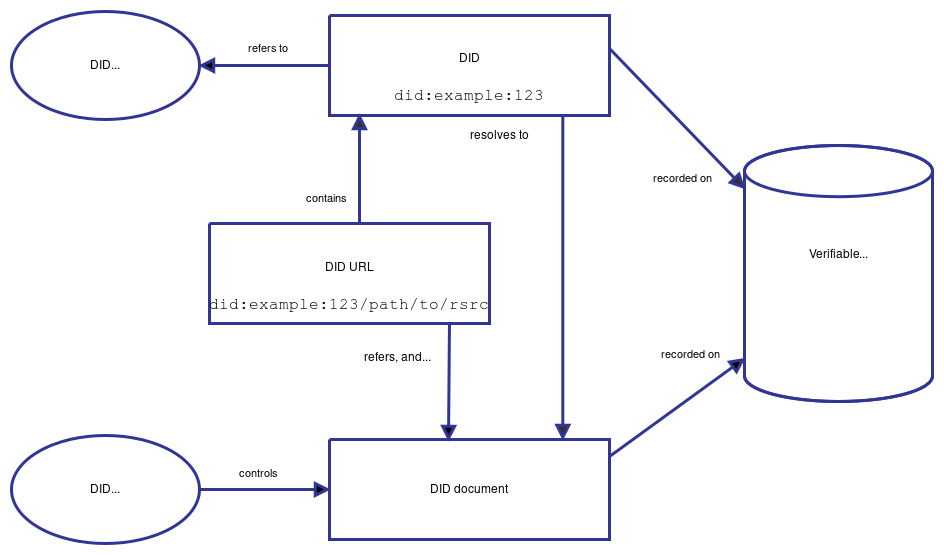
\includegraphics[width=13cm,keepaspectratio]{did-architecture.png}
    \centering
    \caption{Panoramica dell'architettura dei \gls{did} e le relazioni fra le componenti fondamentali \cite{img:did-architecture}}
    \label{lab:did-architecture}
\end{figure}

Il soggetto identificato ha bisogno di un’identità per essere in grado di dimostrare di possedere determinati tratti o caratteristiche a un verificatore. \\
Il verificatore ha un certo numero di emittenti di fiducia ed è disposto ad accettarne i claims, cioè le affermazioni.
Il soggetto può chiedere a uno di questi emittenti di aggiungere una dichiarazione firmata sul proprio documento \gls{did}.
Inoltre, sia l'emittente che il verificatore devono essere in grado di verificare che il soggetto sia effettivamente il proprietario dell'identità.
Ciò si ottiene tramite DIDAuth. \\
Questo processo può assumere molte forme, come specificato nel documento \gls{did}, ma un modo comune è attraverso un challenge inviata dall'emittente o dal verificatore al soggetto,
del quale conoscono la chiave pubblica grazie al DID document, che a sua volta risponderà firmando con la propria chiave privata, dimostrando la propria identità.

\subsubsection {Analogia con il mondo reale}
Si vuole comprare alcool al bar. Per farlo, si deve essere in grado di dimostrare al barista di avere almeno 18 anni. Il barista in questo caso è il verificatore.
Si può dimostrare la richiesta mostrando la propria carta d'identità.
Questa viene rilasciato dal governo, che funge da emittente di fiducia per il barman,
il quale verificherà che il richiedente sia effettivamente la persona raffigurata nella foto e si convincerà che del possesso del requisito della maggiore età.

\begin{figure}[ht]
    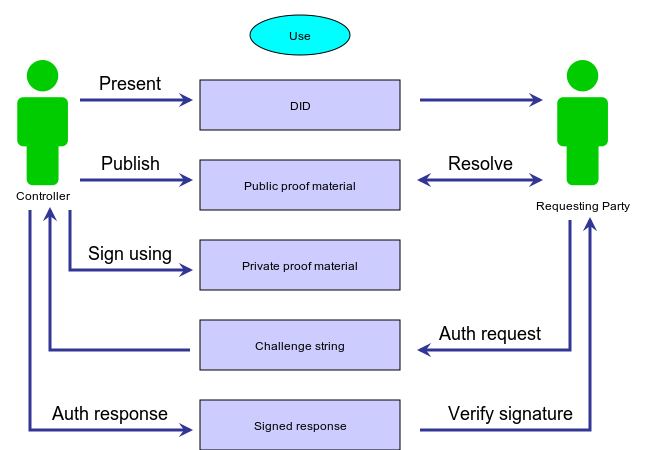
\includegraphics[width=13cm,keepaspectratio]{did-auth.png}
    \centering
    \caption{Panoramica dell'architettura dei \gls{did} e le relazioni fra le componenti fondamentali \cite{img:did-auth}}
    \label{lab:did-auth}
\end{figure}

Le blockchain, grazie alle loro caratteristiche, si sono rivelate un sistema ideale per integrare un sistema di \gls{ssi}, anche in ambiti che esulano il settore energetico \cite{art:blockchain-did}. \\
Nel progetto di \gls{ew} i \gls{did} ricoprono un ruolo centrale.
Ogni utente può richiedere un \gls{did} che mantenga la lista di claims verificabili che l'utente possiede.
È anche possibile assegnare un \gls{did} ad ogni \gls{der}, così da tenere traccia di tutte le informazioni e certificazioni legate a quello specifico \gls{der}. \\

Altri vantaggi forniti da questo sistema sono:
\begin{itemize}
    \item Meccanismo di autenticazione - Il soggetto è in grado di fornire una prova crittografica del proprio controllo sul \gls{did}
    \item Autorizzazione e deleghe -  Il protocollo prevede la possibilità per un \gls{did} di autorizzare o delegare un altro \gls{did} per permettergli di effettuare operazioni a suo nome
\end{itemize}

\section{Identity and Access Management (IAM)}
\label{sec:iam}

\gls{iam} è un insieme di policy in grado di garantire che solo le entità con le credenziali e le autorizzazioni necessarie possano accedere alle risorse. \\
Il sistema deve prima controllare l'identità digitale del soggetto e verificare i ruoli ad esso associati.
L'operazione viene autorizzata solo se il soggetto ha i ruoli necessari.
Per assicurare l'\textit{accountability}, viene utilizzato un sistema di \textit{logging} per registrare ogni operazione eseguita dal soggetto.\\

Per implementare un sistema IAM decentralizzato bisogna garantire alcune proprietà.

\textbf{L'IAM deve essere resistente alla censura.}
Significa che non esiste alcun attore nel sistema che abbia il potere di limitare selettivamente le informazioni a cui gli altri hanno accesso.
Questo aspetto è importante perché informazioni riguardanti situazioni casi in cui un'autorizzazione o una chiave è stata revocata o invalidata o se è stata appena concessa un'autorizzazione devono essere disponibili pubblicamente. \\
Una blockchain, per sua natura, soddisfa questi requisiti. Inoltre, le prove crittografiche contenute nelle transazioni consentono la verifica off-line dei dati.
Le descrizioni dei ruoli sono contenute in uno smart contract ENS, mentre l'avvenuta concessione di un ruolo e i suoi dettagli è annotata nel documento DID dell'utente, mantenuto off-chain.

\textbf{Le informazioni su utenti e ruoli devono essere riservate.}
Nella soluzione di Energy Web, nessuna terza parte dispone dell'elenco completo degli utenti di un'applicazione. \\
Ciò è garantito dal processo di concessione dell'autorizzazione, poiché è l'utente che archivia il claim e ne aggiunge la descrizione sulla blockchain, consentendogli di dimostrare che gli è stato concessa una determinata autorizzazione (\autoref{lab:iam-process}). \\
Poiché si tratta di una operazione svolta dall'utente stesso, i contenuti del ruolo non sono divulgati \cite{img:iam}.
L'unica informazione che un osservatore può raccogliere è che l'utente ha aggiunto un claim al proprio DID document, ma non il contenuto, l'origine o la natura del claim. \\

\begin{figure}[ht]
    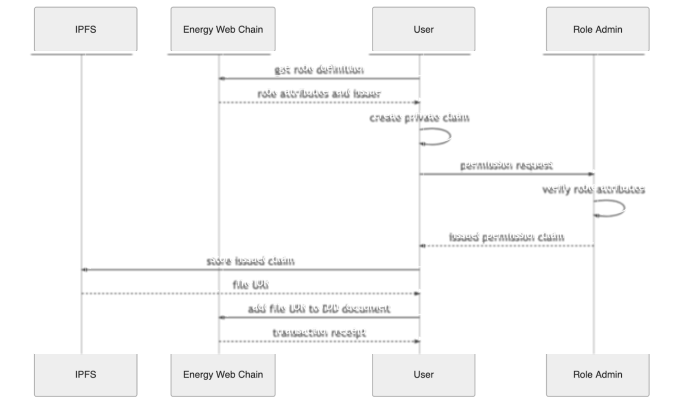
\includegraphics[width=13cm,keepaspectratio]{iam-process.png}
    \centering
    \caption{Processo di rilascio dei ruoli \gls{iam} \cite{img:iam}}
    \label{lab:iam-process}
\end{figure}

Anche l'\gls{iam} rappresenta un punto cardine nel progetto \gls{ew}. \\
Attraverso il suo utilizzo, è possibile creare delle organizzazioni con una struttura gerarchica, simile ai domini attualmente utilizzati sul web.
I ruoli che gli utenti possiedono determinano le azioni che possono compiere all'interno dell'organizzazione. \\
La gestione di tutti questi aspetti è stata resa molto più accessibile grazie alla \gls{dapp} \href{https://switchboard.energyweb.org/}{Switchboard} (\url{https://switchboard.energyweb.org/}).

% Concetti e tecnologie
\chapter{Concetti e tecnologie}

%%%%%%%%%%%%
% Content
%%%%%%%%%%%%
\section{Funzione hash}
Le funzioni hash crittografiche sono una serie di algoritmi che, dato in input una stringa di lunghezza idealmente arbitraria,
restituiscono in output una stringa di bit che rispetta le seguenti caratteristiche:

\begin{itemize}
    \item La lunghezza dell'output è costante
    \item Input identici producono output identici
    \item Un avversario con potenza di calcolo polinomiale che conosca l'output della funzione non è in grado di risalire l'input
    \item L'output deve essere ben distribuito, ovvero deve essere indistinguibile da una distribuzione casuale uniforme
    \item A piccole variazioni nell'input devono corrispondere grandi variazioni nell'output
\end{itemize}

Si noti che ottenere e verificare queste proprietà è un compito molto delicato,
per cui si fa affidamento ad algoritmi e librerie preesistenti con implementazioni sicure, efficienti e testate.


\section{Albero di Merkle}
\label{sec:merkle-tree}
Gli alberi di Merkle (\autoref{lab:merkle-tree}), inventati da Robert Bruce Merkle \cite{art:merkle}, sono un tipo di struttura dati con le seguenti caratteristiche:

\begin{itemize}
    \item Ogni foglia contiene l'hash dell'elemento associato
    \item Risalendo l'albero, ogni nodo contiene l'hash dei due figli
    \item La radice contiene l'hash dell'albero
\end{itemize}

\begin{figure}[h]
    \centering
    \begin{forest}
        for tree={draw,inner sep=10pt,l=20pt,l sep=20pt}
        [
        H(ABCD EFGH)
        [H(AB BC)
                [H(A B)
                        [H(A)]
                            [H(B)]
                    ]
                    [H(C D)
                        [H(c)]
                            [H(D)]
                    ]
            ]
            [H(EF GH)
                [H(E F)
                        [H(E)]
                            [H(F)]
                    ]
                    [H(G H)
                        [H(G)]
                            [H(H)]
                    ]
            ]
        ]
    \end{forest}
    \caption{Albero di Merkle \label{lab:merkle-tree}}
\end{figure}

Utilizzare un albero di Merkle per assicurare l'immutabilità dei dati è una soluzione molto efficace e sicura,
ed rappresenta una strategia molto comune nella realizzazione di architetture distribuite come la blockchain. \\
Un albero di Merkle, infatti, è in grado di provare l'immutabilità di un numero enorme di dati anche molto grandi
mantenendo in memoria solo la radice dell'albero. \\
Inoltre, è possibile verificare l'appartenenza all'albero di uno qualsiasi delle sue foglie rivelando unicamente
il valore della foglia incriminata e gli hash necessari a ricostruire la radice (\autoref{lab:merkle-tree-verify}).
Non è quindi necessario fornire informazioni sulle altre foglie.

\begin{figure}[h]
    \centering
    \begin{forest}
        for tree={draw,inner sep=10pt,l=20pt,l sep=20pt}
        [
        H(ABCD EFGH), fill=green!25
        [H(AB BC), fill=blue!25
        [H(A B)
        [H(A)]
            [H(B)]
        ]
        [H(C D)
        [H(c)]
            [H(D)]
        ]
        ]
        [H(EF GH), fill=green!25
        [H(E F), fill=green!25
        [H(E), fill=red!25]
        [H(F), fill=blue!25]
        ]
        [H(G H), fill=blue!25
        [H(G)]
        [H(H)]
        ]
        ]
        ]
    \end{forest}
    \caption{Per verificare l'appartenenza della foglia \colorbox{red!25}{E} all'albero,
        è necessario fornire unicamente gli \colorbox{blue!25}{hash} dei nodi fratelli.
        Con quelli è possibile ricostruire la \colorbox{green!25}{radice} dell'albero \label{lab:merkle-tree-verify}}
\end{figure}

\section{Metamask}
\label{sec:metamask}
MetaMask è un portafoglio software pensato per interagire con blockchain basate su Ethereum.
Permette a chiunque di partecipare molto comodamente alla blockchain attraverso un estensione browse o un'app mobile. \\
Nel concreto, MetaMask permette agli utenti di memorizzare le proprie chiavi private direttamente nell'estensione,
permettendo poi agli sviluppatori di interagire con le sue \gls{api}.
Ciò consente, ad esempio, di creare in maniera sicura transazioni da inviare agli altri nodi della blockchain. \\
Sebbene i più critici possano rimanere contrariati dalla fiducia riposta in questo tipo di software, la sua adozione
è sempre più comune.

% Progetto
\chapter{Progetto}

\section{Architettura}
La soluzione proposta si avvale di una architettura ibrida, che prova a conciliare le i servizi e le opportunità
che l'utilizzo della blockchain offre con le sue limitazioni intrinseche. \\
Piuttosto che provare ad abbracciare a tutti i costi un modello esclusivamente distribuito, si è optato per
mantenere un approccio più tradizionale per quanto riguarda l'immagazzinamento e la gestione dei dati. \\

Si individuano quindi i seguenti agenti (\autoref{lab:did-architecture}):
\begin{itemize}
    \item un numero arbitrario di \gls{der} che fa capo ad un \gls{prosumer}
    \item un numero arbitrario di \gls{prosumer} che fa capo ad un \gls{aggregator}
    \item un \gls{aggregator}
    \item una DApp, che fornisce un'interfaccia per per consultare i dati
\end{itemize}

\begin{figure}[h]
    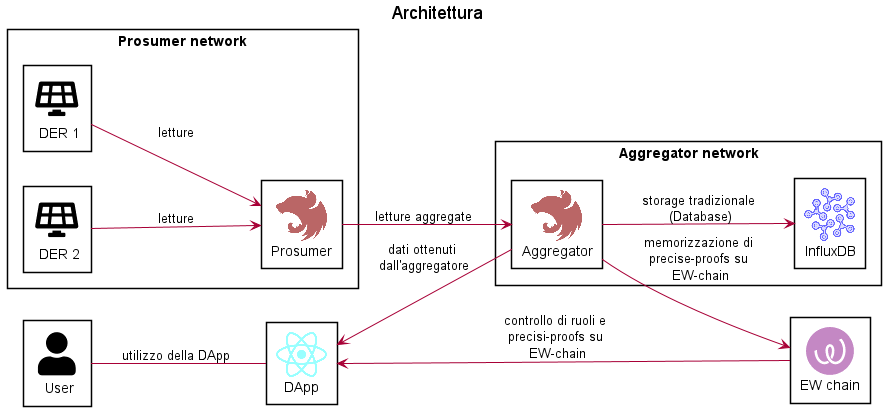
\includegraphics[width=\linewidth,keepaspectratio]{diagram-architecture.png}
    \centering
    \caption{Un esempio di architettura che include un \gls{prosumer} che possiede due \gls{der} ed un \gls{aggregator}}
    \label{lab:diagram-architecture}
\end{figure}

Al \gls{prosumer} si assegna un ruolo di rilievo, in quanto responsabile per la creazione delle precise-proof
che garantiscono l'integrità e il non ripudio dei dati. 
Queste responsabilità aggiuntive attribuite al singolo utente rappresentano uno degli aspetti chiave di questo approccio. \\
\\
All'\gls{aggregator} spetterà il compito di verificare la correttezza e la validità dei dati acquisiti,
sfruttando varie tecnologie crittografiche e i servizi offerti da \gls{ew}.
Se la validazione va a buon fine, i dati vengono salvati su un database tradizionale. \\
Contemporaneamente viene eseguito un apposito metodo sullo smart contract designato sulla blockchain,
che emetterà un log con il DID dell'\gls{aggregator} e la precise-proof associata alle letture. (\autoref{lab:diagram-flow-aggregator})\\

\begin{figure}[H]
    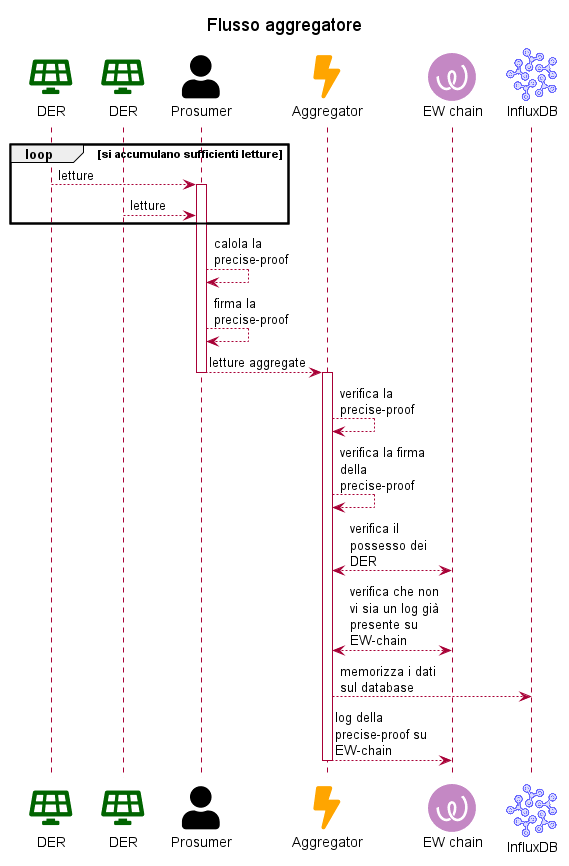
\includegraphics[scale=0.5]{diagram-flow-aggregator.png}
    \centering
    \caption{Diagramma di sequenza che del flusso per la registrazione di nuove letture}
    \label{lab:diagram-flow-aggregator}
\end{figure}

Una possibile interfaccia, realizzata tramite DApp, può sfruttare il sistema di \gls{iam} offerto da \gls{ew}
per consentire l'accesso e la visualizzazione dei dati richiedendo un'autenticazione minimale,
che viene delegata alla crittografia asimmetrica usata tradizionalmente sulle blockchain (\autoref{lab:diagram-flow-dapp}). \\


\begin{figure}[H]
    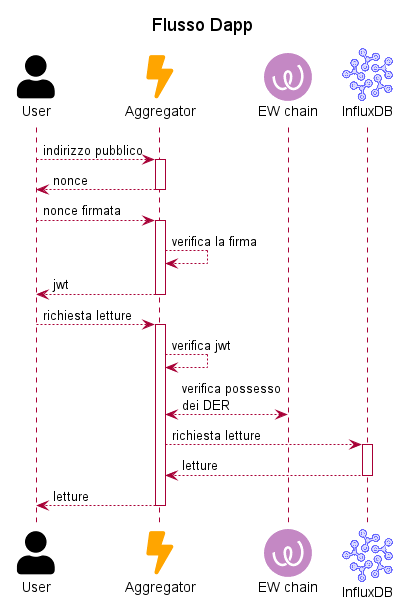
\includegraphics[scale=0.5]{diagram-flow-dapp.png}
    \centering
    \caption{Diagramma di sequenza del flusso per la lettura di dati dall'\gls{aggregator}}
    \label{lab:diagram-flow-dapp}
\end{figure}


\section{Componenti}

\subsection{DER}
I protagonisti del progetto sono proprio i DER, in una visione che li vuole identificare come dispositivi \gls{iot} piuttosto semplici.
L'unico requisito che devono soddisfare i DER è di avere una connessione alla rete locale per poter utilizzare il protocollo \gls{http}. \\
Le letture possono essere effettuate ad una cadenza arbitraria stabilita dall'\gls{oem} o dall'ente competente che ha installato il dispositivo. \\
Il dispositivo ha volutamente un ruolo molto limitato. Non è necessario che sia a collegato con altri \gls{der}
o che possieda ulteriori informazioni oltre quelle prodotte dal suo funzionamento e il \gls{did} che lo identifica. \\
L'unica comunicazione che il dispositivo effettua tramite la rete locale è verso l'applicazione del \gls{prosumer}.
Non è necessario sia connesso alla rete internet perché il protocollo funzioni. \\
Il payload (\autoref{lab:der-payload}) inviato è estremamente semplice e contiene solo le informazioni essenziali,
quali il \gls{did} del dispositivo, il timestamp e il valore registrato con la lettura, compresa l'unità di misura. \\

\begin{listing}
    \begin{minted}{json}
{
    "assetDID": "did:ethr:0x0000000000000000000000000000000000000000",
    "timestamp": "2020-01-01T00:00:00Z",
    "value": 100,
    "unit": "Wh"
}
\end{minted}
    \caption{Esempio di payload mandato dal \gls{der} all'\gls{prosumer}}\label{lab:der-payload}
\end{listing}

Il \gls{der} può essere simulato con l'invio periodico dei dati al \gls{prosumer} locale tramite uno script come questo:
\inputminted[linenos]{bash}{../der/iot_source.sh}

\subsection{Prosumer}
\label{sec:prosumer}

Il \gls{prosumer} in questo contesto si riferisce ad un'applicativo che ha il compito
di mettere insieme le letture provenienti da più \gls{der} della \gls{lan} a cui appartiene. \\
Il \gls{prosumer} è una applicazione web che espone una semplice \gls{api} \gls{rest} attraverso la quale ricevere le letture dei \gls{der}, accumulandole. \\
Dopo aver raggiunto un numero sufficiente di letture, che in questo caso sono banalmente memorizzate in un database
SQLite\cite{sftw:sqlite}, il \gls{prosumer} crea una precise-proof che le vincola. \\
Il vantaggio di usare una precise-proof basata sulla radice di un albero di Merkle (cfr. \autoref{sec:merkle-tree}) è che,
qualora fosse necessario dimostrare di aver effettuato e comunicato correttamente una lettura specifica all'\gls{aggregator},
sarà sufficiente mostrare il singolo dato incriminato e fornire gli hash dei nodi adiacenti necessari a ricostruire l'albero,
riducendo in modo significativo la quantità di dati potenzialmente sensibili da condividere. \\
Il \gls{prosumer} firmerà poi con la sua chiave privata la precise-proof. \\
Ciò fornisce all'\gls{aggregator} una garanzia sul proprio interlocutore e protegge la precise-proof, e quindi l'intero payload,
da possibili alterazioni. \\
Viene quindi costruito un payload (\autoref{lab:prosumer-payload}) che contiene la lista di tutti i dati e il valore della precise-proof.
A ciò si aggiunge la lista dei valori di salt \cite{wiki:salt} utilizzati nella creazione dell'albero e la firma digitale applicata alla precise-proof, e qualche informazione di comodità
come i timestamp della prima e ultima lettura. \\
Dopo aver mandato il proprio payload, interfacciandosi direttamente con la \gls{ewc} è possibile captare i log prodotti dallo smart contract di riferimento
che contengono la precise-proof contenuta nel payload.
Una volta ricevuto il log, si ha la garanzia che tutto il flusso è andato a buon fine e che la precise-proof rimarrà perennemente registrata e consultabile.

\begin{listing}[h]
    \begin{minted}{json}
{
    "start": "2022-01-01T00:00:00Z",
    "stop": "2022-01-02T00:00:00Z",
    "rootHash": "09urv0un981evup2m8u3",
    "salts": [
        "salt1",
        "salt2"
    ],
    "status": "NotSubmitted",
    "readings": [
        {
            "assetDID": "did:ethr:0x0000000000000000000000000000000000000000",
            "timestamp": "2022-01-01T00:00:00Z",
            "value": 10000000,
            "unit": "Wh"
        },
        {
            "assetDID": "did:ethr:0x0000000000000000000000000000000000000000",
            "timestamp": "2022-01-02T00:00:00Z",
            "value": 1000,
            "unit": "Wh"
        }
    ],
    "signature": "signed root hash"
}
\end{minted}
    \caption{Esempio di payload mandato dal \gls{prosumer} all'\gls{aggregator}}\label{lab:prosumer-payload}
\end{listing}

\subsection{Aggregator}
L'\gls{aggregator} offre un servizio pubblico a cui i \gls{prosumer} della sua giurisdizione fanno riferimento.
Il suo ruolo è principalmente di controllo, e si limita a raccogliere i dati che riceve, verificare che siano corretti e
assicurarsi che il mittente sia autorizzato a compiere questa azione. \\
Ciò viene fatto in un primo luogo verificando la firma digitale della precise-proof.
Successivamente viene ricostruito l'albero di Merkle a partire dalle letture e dai salt e si verifica che la precise-proof corrisponda.
Per finire, viene consultata la \gls{ewc} per controllare che il mittente sia anche il proprietario di tutti i \glsplural{der} che figurano nelle letture. \\
Se tutti questi controlli sono andati a buon fine, le informazioni sono salvate in un database InfluxDB \cite{sftw:influxdb}, un software specializzato nell'immagazzinamento di dati sotto forma di serie storiche.
Infine viene chiamato il metodo il metodo \textbf{store} sullo smart contract \textbf{ReadingsNotary} (\autoref{lab:readings-notary}), attualmente presente su Volta all'indirizzo \href{https://volta-explorer.energyweb.org/address/0xe574fDD8C3148f2E883612A9C6CDA7b9C12d1566/transactions}{0xe574fdd8c3148f2e883612a9c6cda7b9c12d1566}.

\begin{listing}[h]
    \begin{minted}{solidity}
// SPDX-License-Identifier: MIT
pragma solidity 0.8.4;

contract ReadingsNotary {
    /** A new metered reading has been emitted */
    event NewMeterReading(address indexed operator, bytes indexed proof);

    /** Store a new reding
     * @param _proof Merkle root of the tree of merkle proofs of the aggregated readings
     */
    function store(bytes calldata _proof) external {
        emit NewMeterReading(msg.sender, _proof);
    }
}
\end{minted}
    \caption{Smart contract \textbf{ReadingsNotary}, rilasciato su Volta all'indirizzo \textit{0xe574fdd8c3148f2e883612a9c6cda7b9c12d1566}}\label{lab:readings-notary}
\end{listing}

L'\gls{aggregator} fornisce pubblicamente una interfaccia \gls{api} \gls{rest} che consente di accedere ai dati memorizzati al fine di consultarli.
L'accesso è protetto da un sistema di autenticazione che si svolge in due fasi:

\begin{enumerate}
    \item Si richiede una nonce generata sul momento dal \gls{aggregator} associandola alla propria chiave pubblica
    \item Si invia la firma digitale della nonce al passaggio precedente, ottenendo un \gls{jwt} con validità di 24 ore dall'\gls{aggregator}
\end{enumerate}

Un utente ha accesso solo ai dati relativi ai \gls{did} che possiede.
Fa eccezione l'utente \gls{aggregator}, che può accedere a tutti i dati memorizzati nel database.

\subsection{DApp}
Il \gls{dapp} è una applicazione web che consente di accedere ai dati memorizzati dall'\gls{aggregator}.
Il login viene effettuato tramite Metamask (cfr. \autoref{sec:metamask}).
Si ha quindi la possibilità di firmare la nonce per autenticarsi con il server dell'\gls{aggregator}. \\
Una volta effettuato l'accesso, la web app verifica automaticamente i claim associati ad \gls{did} dell'utente
che ha eseguito il login, che potrebbe possedere il ruolo di \gls{aggregator}. \\

\subsubsection{Aggregator}
Se l'utente è un \gls{aggregator}, gli verrà mostrata un interfaccia che gli permette di visualizzare, tramite un grafico,
la produzione o il consumo di tutti i \gls{der} registrati nel suo database (\autoref{lab:dapp-prosumer-readings}).
Aggregando i dati provenienti da più fonti, è possibile avere una visione chiara dello stato della rete elettrica
nella finestra temporale specificata. Ciò permette di evidenziare facilmente anomalie o situazioni di penuria o sovrabbondanza
di energia elettrica. \\
Questo tipo di monitoraggio potrebbe essere uno strumento in più per permettere un intervento tempestivo in situazioni che lo richiedano. \\
Basandosi sui dati aggiornati e aggregati secondo una metrica stabilita, l'\gls{aggregator} è inoltre in grado di abbinare domanda e offerta (\autoref{lab:dapp-aggregator-match}). \\

\begin{figure}[H]
    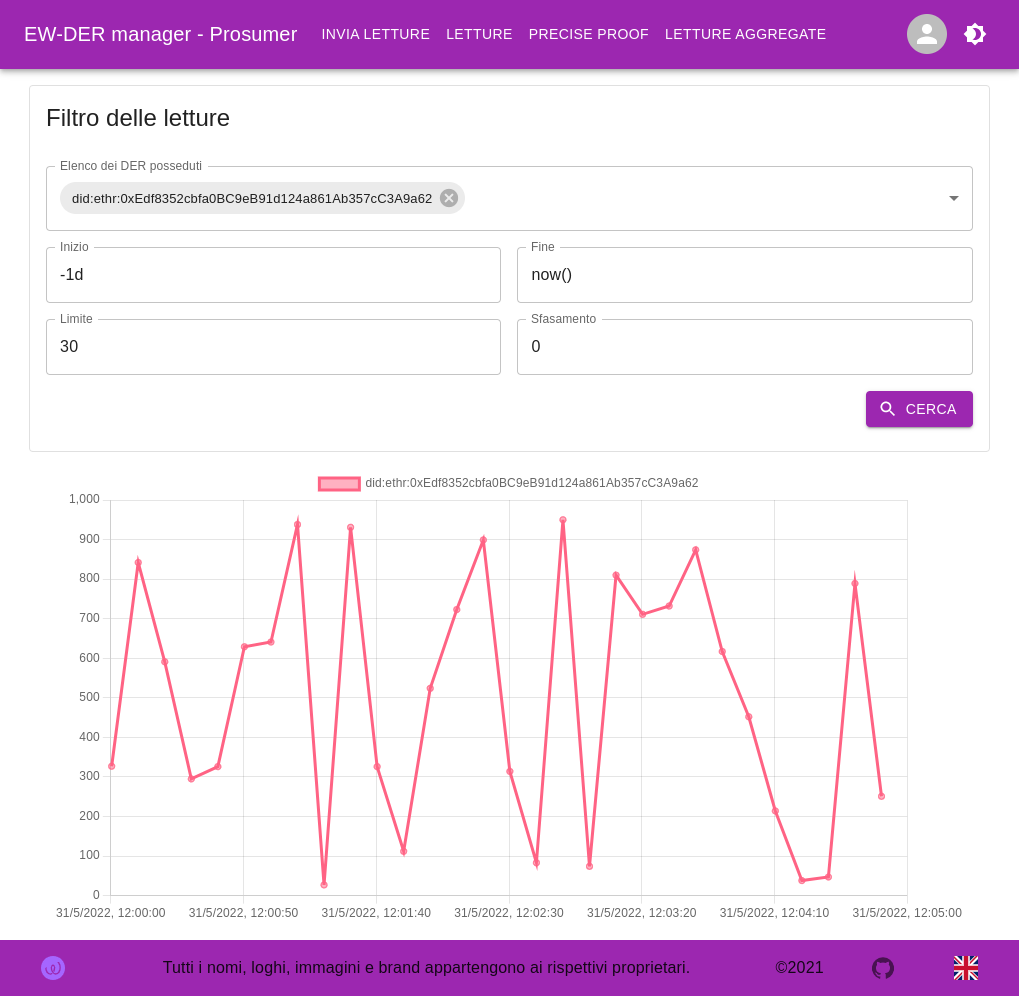
\includegraphics[width=0.72\linewidth,keepaspectratio]{dapp-prosumer-readings.png}
    \centering
    \caption{Schermata che permette al \gls{prosumer} visualizzare le letture dei propri \gls{der}. L'\gls{aggregator} ha a disposizione la stessa schermata, ma può richiede informazioni su un qualsiasi \gls{der}}
    \label{lab:dapp-prosumer-readings}
\end{figure}

\begin{figure}[H]
    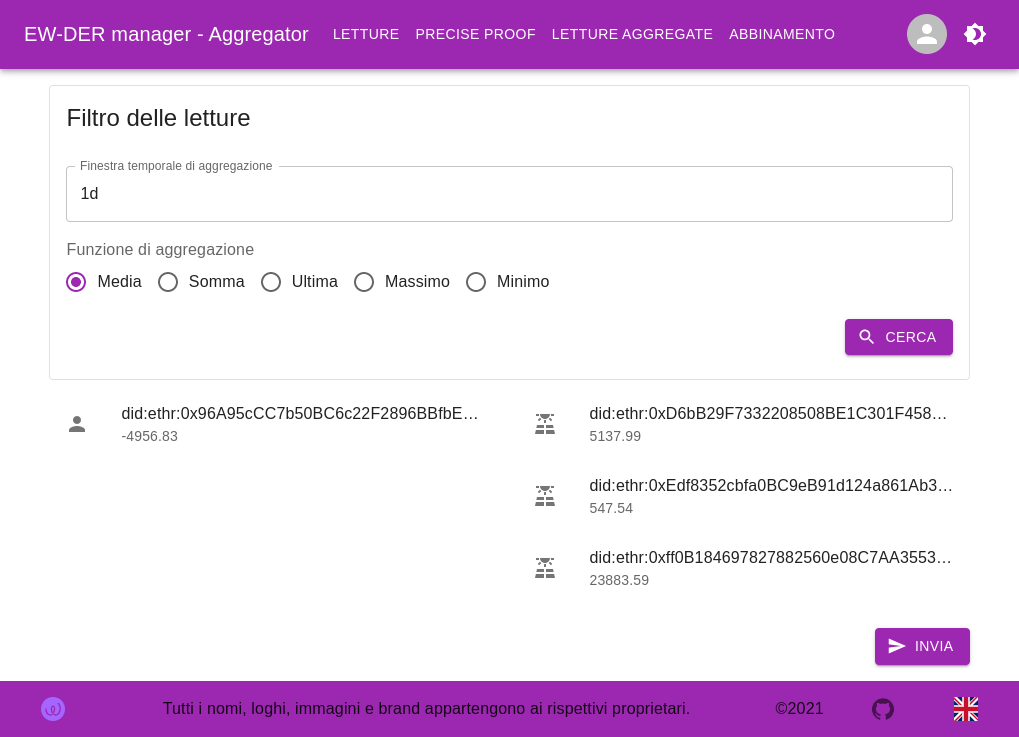
\includegraphics[width=0.72\linewidth,keepaspectratio]{dapp-aggregator-match.png}
    \centering
    \caption{L'\gls{aggregator} associa domanda e offerta in base ai dati recenti memorizzati}
    \label{lab:dapp-aggregator-match}
\end{figure}

\subsubsection{Prosumer}
Se l'utente è un \gls{prosumer}, è in grado di consultare i dati memorizzati dall'\gls{aggregator} e visualizzarli tramite un grafico. \\
Ai fini della demo, l'utente sarà anche in grado di inviare una serie fittizia di letture aggregate appartenenti a dei \gls{der} che possiede. \\
L'invio delle letture segue i passaggi indicati precedentemente (cfr. \autoref{sec:prosumer})

\begin{figure}[H]
    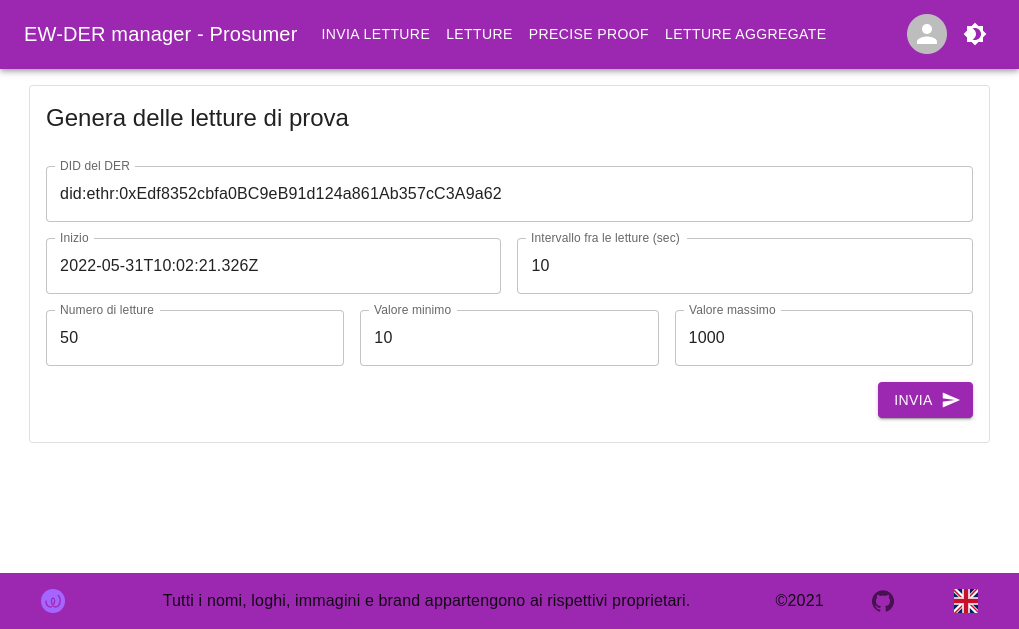
\includegraphics[width=0.72\linewidth,keepaspectratio]{dapp-prosumer-generate.png}
    \centering
    \caption{Schermata che permette al \gls{prosumer} di simulare l'invio di letture all'\gls{aggregator}}
    \label{lab:dapp-prosumer-generate}
\end{figure}

\section{Implementazione}

\subsection{Materiale disponibile}
L'implementazione di tutte le componenti descritte in questa sezione è pubblicamente consultabile all'indirizzo \href{https://github.com/TendTo/EW-DER-API}{https://github.com/TendTo/EW-DER-API}. \\
Leggendo i file \textit{README.md}, presenti in quasi tutte le sottocartelle, è possibile farsi un'idea dei requisiti e delle configurazioni necessarie
ad avviare quella sezione dell'architettura. \\

Sulla blockchain Volta sono stati inoltre rilasciati i seguenti smart-contract:

\begin{itemize}
    \item \textbf{Multicall} (\href{https://volta-explorer.energyweb.org/address/0xEe2ADcB5BEAa7E08AF1F1a4Ee0EFfE0DfDDEdD27/contracts}{\textbf{0xEe2ADcB5BEAa7E08AF1F1a4Ee0EFfE0DfDDEdD27}}): smart contract standard usato per ottimizzare multiple chiamate a funzioni costanti, aggregandole in un'unica operazione \cite{sftw:multicall}
    \item \textbf{Readings notary} (\href{https://volta-explorer.energyweb.org/address/0xe574fDD8C3148f2E883612A9C6CDA7b9C12d1566/contracts}{\textbf{0xe574fDD8C3148f2E883612A9C6CDA7b9C12d1566}}): smart contract usato dall'\gls{aggregator} per produrre i log delle letture
\end{itemize}

Una demo della \gls{dapp} è disponibile all'indirizzo \href{https://tendto.github.io/EW-DER-API/}{https://tendto.github.io/EW-DER-API/} \\
Per poterla provare di persona è necessario:
\begin{itemize}
    \item installare \href{https://metamask.io/}{Metamask}
    \item connettere Metamask alla blockchain Volta seguendo i passaggi indicati nella \href{https://energy-web-foundation.gitbook.io/energy-web/how-tos-and-tutorials/connect-to-energy-web-chain-main-network-with-metamash}{documentazione} fornita da \gls{ew}
    \item assicurarsi di avere a disposizione qualche Volta Token, che è possibile ottenere dall'apposito \href{https://voltafaucet.energyweb.org/}{faucet}
\end{itemize}


\subsection{\glsfirst{bom}}
Al fine di realizzare tutte le componenti di questa architettura sono state utilizzate le seguenti librerie, framework e tecnologie:

\begin{itemize}
    \item \textbf{SQLite} \cite{sftw:sqlite}: implementazione di un SQL database engine piccolo, veloce ed affidabile
    \item \textbf{InbluxDB} \cite{sftw:influxdb}: database specializzato per immagazzinare dati sotto forma di serie storiche
    \item \textbf{NestJS} \cite{sftw:nestjs}: framework javascript per la creazione di applicazioni web back-end
    \item \textbf{hardhat} \cite{sftw:hardhat}: framework javascript per la creazione e il deploy di smart contracts su blockchain
    \item \textbf{iam-client-lib} \cite{sftw:iam-client-lib}: libreria javascript realizzata da \gls{ew} usata per interagire con il loro servizio di \gls{iam}
    \item \textbf{react} \cite{sftw:react}: framework javascript per la creazione di applicazioni web
    \item \textbf{ethers} \cite{sftw:ethers}: libreria javascript usata per interfacciarsi con la blockchain
\end{itemize}

\subsection{Setup locale}
Per ottenere una simulazione fedele di più componenti che interagiscono fra loro in un sistema distribuito come quello proposto e
per offrire la possibilità di ricreare l'intera architettura facilmente e senza requisiti complessi, è stato utilizzato il sistema di containerizzazione Docker \cite{sftw:docker}. \\
La repository git contiene un file \textit{docker/docker-compose.yml} utilizzabile per inizializzare tutti i container necessari per l'esecuzione dell'architettura.
Sebbene la maggior parte dei parametri di default sia adatta alla maggior parte dei casi d'uso, ve ne sono alcuni che è necessario sovrascrivere. \\
Poiché si tratta di dati sensibili, è consigliabile creare nella stessa cartella un file \textit{docker/docker-compose.override.yml} (\autoref{lab:docker-compose-override}) contenente i parametri da sovrascrivere,
per evitare di renderli pubblici accidentalmente.

\begin{listing}[H]
    \begin{minted}{yaml}
version: "3.9"

services:
  aggregator:
    environment: # Chiave segreta o mnemonic dell'aggregatore. Assicurarsi di avere a disposizione qualche Volta token
      SK: swear fest avoid yolk cat dog tagging water bag coat wardrobe

  prosumer:
    environment: # Chiave segreta o mnemonic del prosumer
      SK: cable fest scissor slide pen smart picture oil water bag coat cup
\end{minted}
    \caption{Esempio di \textit{docker/docker-compose.override.yml}}\label{lab:docker-compose-override}
\end{listing}

Per avviare l'intero stack, eseguire il comando \mintinline{bash}{$ docker-compose up} nella directory \textit{docker}. \\
Per fermare l'esecuzione, eseguire \mintinline{bash}{$ docker-compose down}. \\
Per rimuovere i volumi Docker rimasti, eseguire \mintinline{bash}{$ docker volume prune}. \\
Se si vuole avere a disposizione anche la \gls{dapp} come interfaccia grafica, questa può essere avviata in locale 
installando le dipendenze necessarie con \mintinline{bash}{$ npm install} e eseguendo \mintinline{bash}{$ npm start}, il tutto nella cartella \textit{app}.
Si possono specificare alcuni parametri di configurazione creando un file \textit{.env} contenente le seguenti chiavi:

\begin{listing}[H]
    \begin{minted}{bash}
PORT=3005
REACT_APP_API_URL=https://ew-der-api.azurewebsites.net
\end{minted}
    \caption{Esempio di \textit{docker/docker-compose.override.yml}}\label{lab:docker-compose-override}
\end{listing}


% Conclusione
\chapter*{Conclusione}
\addcontentsline{toc}{chapter}{Conclusione} % add the chapter to the index
È ragionevole assumere che la decentralizzazione della rete elettrica sia un processo inevitabile che coinvolgerà un numero sempre crescente di utenze,
sia nel ruolo di consumatori che nel ruolo di produttori. \\

Fra le possibili soluzioni, quella di usare la blockchain come infrastruttura in grado di supportare questo mercato sempre più decentralizzato sembra essere particolarmente promettente. \\
Ad una analisi approfondita \gls{ew} risulta essere un progetto con una visione ed un focus chiari, guidato da persone che hanno le conoscenze necessarie per creare una piattaforma ad hoc per questo settore. \\
Proprio in virtù di ciò, le tecnologie che \gls{ew} impiega non sono necessariamente innovative.
Si cerca, al contrario, di seguire ed implementare quanti più standard possibile, e partire da questi per fornire dei servizi che rendano appetibile l'intera infrastruttura. \\
La scelta di rendere tutto il materiale, le implementazioni e le librerie open-source è in linea con la volontà di fornire degli strumenti che facilitino la vita agli sviluppatori,
sui quali poi ricade il compito di creare \gls{dapp} e servizi per l'utente finale. \\
È bene, infine, tenere a mente che \gls{ew}, al momento della stesura di questo documento, è un progetto in divenire, e, per questo, soggetto a continui cambiamenti.
Nonostante ciò, penso che \gls{ew} fornisca quantomeno un ottimo caso di studio che valga la pena approfondire per chi fosse interessato ad affrontare la problematiche trattate nell'introduzione del documento.


% Bibliografy
\printglossary
\printbibliography

\end{document}
